\documentclass[11pt,twocolumn]{article}

\usepackage{graphicx} % for pdf, bitmapped graphics files
\usepackage{times} % assumes new font selection scheme installed
\usepackage{titling}
\usepackage[a4paper, total={7in, 10in}]{geometry}
\usepackage{cuted}
\usepackage{capt-of}
\usepackage[format=plain,
            labelfont=it,
            textfont=it]{caption}
\usepackage{sectsty}
\subsectionfont{\normalfont\itshape}
\usepackage[compact]{titlesec}
\titleformat*{\section}{\Large\bfseries\sffamily}

\setlength\parindent{0pt}
\setlength{\parskip}{1em}

\title{\textbf{Benchmark the Fault-tolerant Mechanism on Hadoop MapReduce Framework}}
\author{Heting Wang\thanks{heting.wang@ufl.edu} \and Eakta Jain\thanks{ejain@cise.ufl.edu}}

\providecommand{\keywords}[1]
{
  \textbf{Keywords:} #1
}
\providecommand{\concepts}[1]
{
  \textbf{Concepts:} #1
}

\begin{document}
\maketitle
\begin{strip}\centering
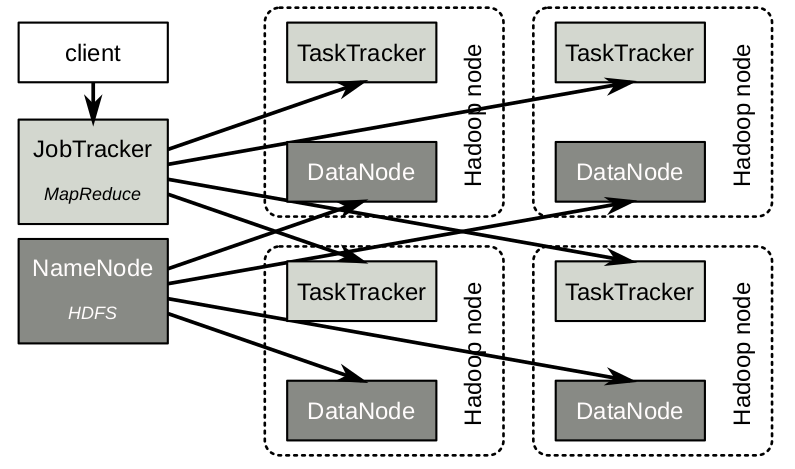
\includegraphics[width=0.5\textwidth]{architecture}
\captionof{figure}{The typical architecture of Hadoop Mapreduce framework.
\label{fig:architecture}}
\end{strip}

\begin{abstract}
Distributed file systems (DFS) with the technique of distributed stream processing\cite{cherniack2003scalable} have been used widely in the real world because they have multiple benefits such as the flexibility of managing resources, easy to access and maintain, and relatively high fault-tolerant capability\cite{schneider1990implementing}. It is essential to remain system robust as arbitrary defects may occur at any part of the low-level system. The goal of this research is to provide a quantitative measurement for fault-tolerant DFS to help users find the most reliable method under their working conditions. We proposed a comparable overview of the current system reliability improvement mechanisms on two distributed MapReduce frameworks\cite{condie2010mapreduce,dean2010mapreduce} built on HDFS: Apache Hadoop\cite{5496972} and Apache Spark\cite{zaharia2010spark,Zaharia:2016:ASU:3013530.2934664}. Then benchmarked the system performance of the Hadoop MapReduce framework after modifying the replication factor from 2 to 3.
Results show that this more reliable system still shows relatively the same good performance compared with the original system.
\end{abstract}

\keywords{distributed file systems, Hadoop MapReduce}

\concepts{$\bullet$\textbf{Benchmark}$\rightarrow$\textbf{Test system performance}}


\section{Introduction}
As big data analysis becomes a hot spot in this information explosion era, every researcher in this field needs to have the ability to extract and process a large amount of data. However, a large dataset in the real world is very difficult to filter and manage valuable information manually on a single machine. Fortunately, with the help of existing data processing frameworks, if we input these large datasets in terms of splits to clusters which consist of one NameNode and multiple DataNodes, the processing time can be reduced to one day or even less. The parameter tuning and model optimization procedure also become simpler. Thus the time consuming and programming difficulty problems can be solved. \par

Though the large-scale DFS has been widely used, there are still not enough research papers focusing on the testing of these fault-tolerant systems and the result analysis. Previously published papers also need to be updated by the newest techniques that came out in recent years. Our study is not focusing on designing fault-tolerant models on DFS, instead, we are concerning how the system will be influenced after setting up the fault-tolerant models. In our experiment, we applied the method of data replication as a fault model on the well-known Hadoop MapReduce framework, aiming at constructing a more comprehensive evaluation of reliable system performance.
\section{Background/Related Work}
Hadoop and Spark MapReduce are both popular highly scalable data processing architectures with strong community supports\cite{ranger2007evaluating,zaharia2008improving}, many researchers have developed efficient methods to enhance iterative MapReduce computations\cite{bhatotia2011incoop,ekanayake2010twister,ekanayake2008mapreduce,fadika2010lemo}, which made them became good prototypes to develop fault-tolerant models.\par

The key difference between them lies in the approach of processing: Spark can do it in-memory, while Hadoop MapReduce has to read from and write to a disk. As a result, the speed of processing differs significantly – Spark may be up to 100 times faster. However, the volume of data processed also differs: Hadoop is able to work with far larger datasets than Spark. 
\subsection*{Hadoop MapReduce}
Hadoop is the base platform on which we run our experiments. In a Hadoop MapReduce application, the user specifies a map function that processes data files to generate a set of intermediate key/value pairs, and a reduce function then merges all intermediate values associated with the same intermediate key. Many real-world tasks are expressible in this model, as illustrated in\cite{62}. Hadoop MapReduce runs on the Hadoop Distributed File System (HDFS), a primary data storage system used by Hadoop applications. It employs a NameNode and DataNode architecture to construct a DFS that provides high-performance access to data across highly scalable Hadoop.\par

HDFS is specially designed to be highly fault-tolerant. By building fault tolerance into every layer of its stack, it hides the complexity of detection and recovery from hardware faults from users\cite{vavilapalli2013apache}. The file system replicates, or copies, each piece of data multiple times and distributes the copies to individual nodes, placing at least one copy on a different server rack than the others. As a result, the data on nodes that crash can be found elsewhere within a cluster. This ensures that processing can continue while data is recovered.\par

The HDFS supports applications with large datasets. Figure \ref{fig:architecture} indicates a common Hadoop architecture, jobs are submitted to the JobTracker located at NameNode and then split into multiple tasks, and these tasks are evenly allocated to different TaskTrackers at distinct DataNodes. Figure \ref{fig:snapshot} shows a snapshot of the web portal when a  program running on nine nodes to count word appearance frequencies in a TXT file.
\begin{figure}[ht]
    \centering
        \includegraphics[width=\linewidth]{Screenshot}
        \caption{The web portal when a Hadoop MapReduce program is running on nine nodes.}
        \label{fig:snapshot}
\end{figure}
\begin{figure}[ht]
    \centering
   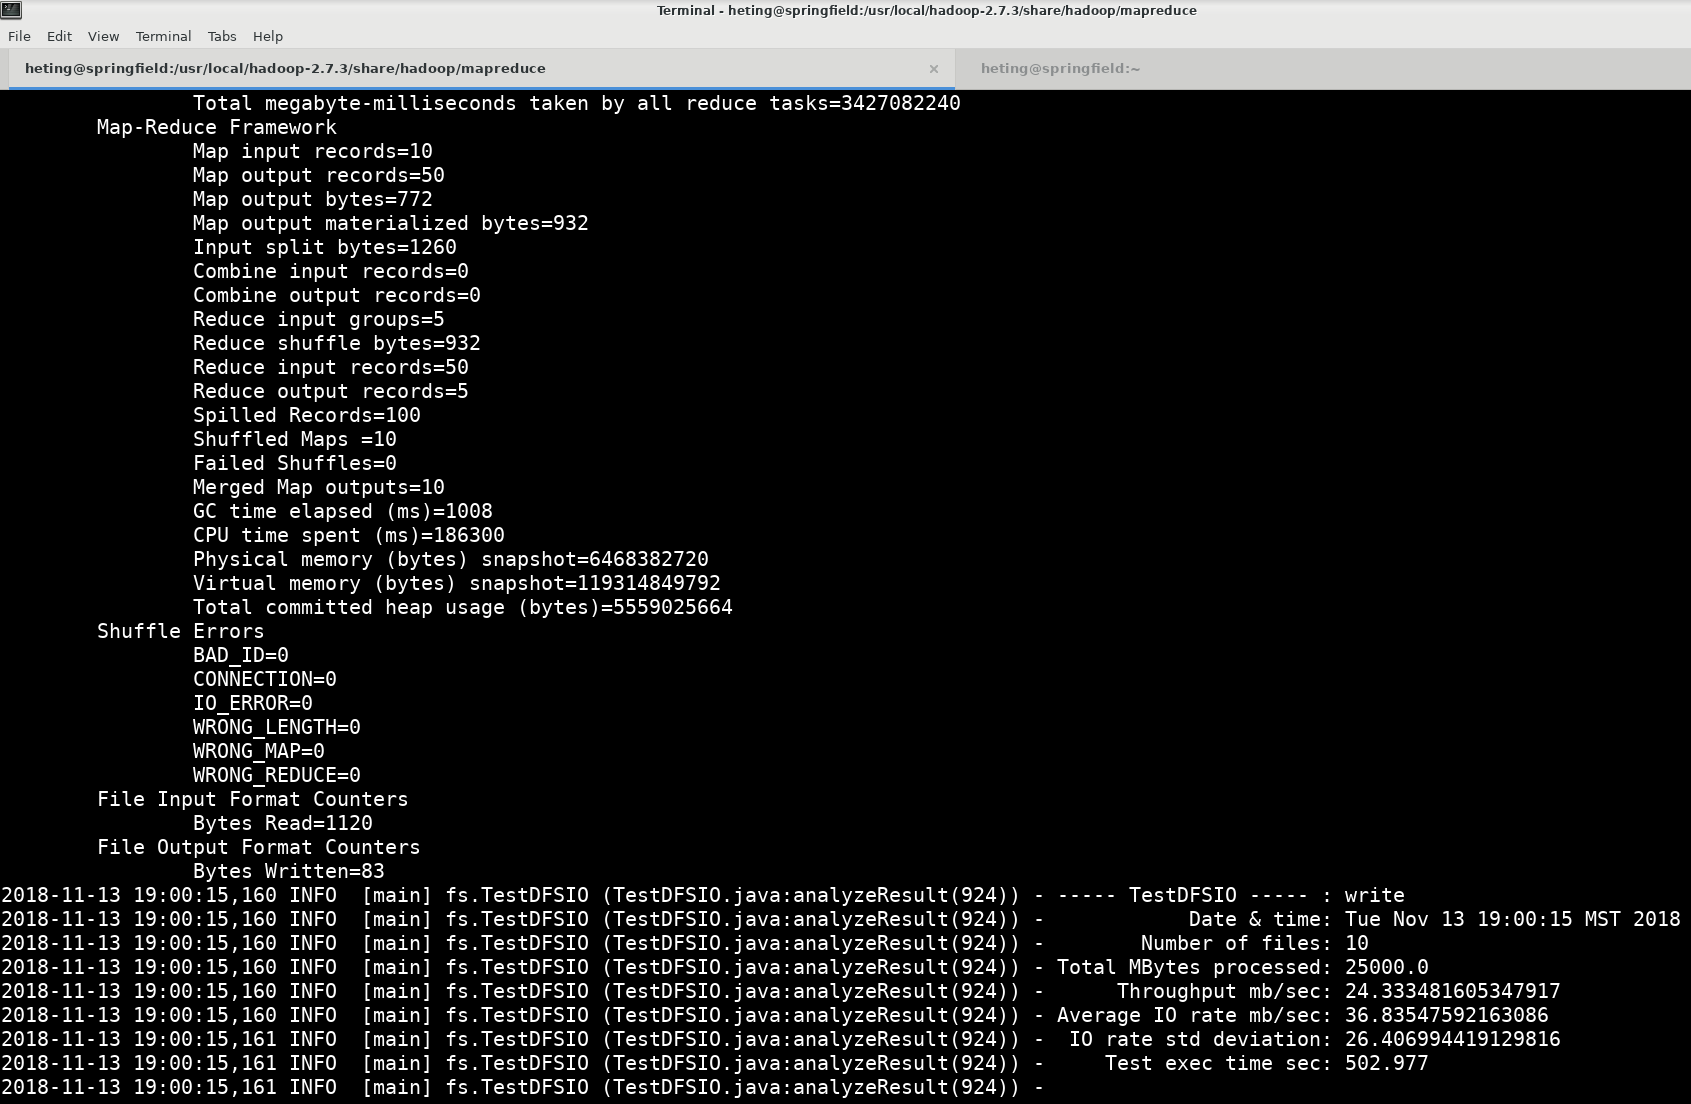
\includegraphics[width=\linewidth]{hadoop}
        \caption{The terminal output after a MapReduce program runs.}
        \label{fig:hadoop}
\end{figure}
Figure \ref{fig:hadoop} presents the terminal output at the end of the running process. The map and reduce task execution conditions can be observed on the screen, as well as whether there exist dead nodes or unsuccessful tasks in the processing duration so that users can better monitor jobs without checking the web portal status all time.

\subsection*{Spark MapReduce}

In Spark, the system builds a lineage chain and the computation is carried out on different clusters depending on actions. The performance of the framework on Spark has been optimized 100 times than Hadoop by using in-memory computation and other optimization. There are two types of operations in Spark: transformations, which perform operations on an input resilient distributed dataset (RDD) to produce one or more new RDDs, and actions, which launch the series of transformations to return the final result. The RDD mentioned here refers to a fundamental data structure in Spark which can be any type of Python, Java, or Scala objects, including user-defined classes in applications\cite{zaharia2012resilient}. An example of the core RDD implementation is shown in figure \ref{fig:example}.
\begin{figure}[ht]
    \centering
        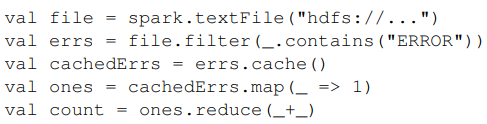
\includegraphics[width=\linewidth]{example}
        \caption{A simple RDD example\cite{zaharia2010spark}.}
        \label{fig:example}
\end{figure}

Most of the fault-tolerant techniques were divided into two methods: focusing on the data duplication at different locations, or rollback, which means saving checkpoints and then recover from the failure point\cite{bala2012fault,patil2013hadoop}. For replication, past research had compared the performance and storage requirements of two data reliability techniques on two open-source systems: HDFS\cite{borthakur2007hadoop} and Ceph. As mentioned in\cite{Arafa:2018:EFT:3219104.3229269}, to maintain fault-tolerance ability, replication and erasure coding (EC) had been used on this two DFS. Another research proposed heuristics to schedule backups, move backup instances, and select backups upon failure for fast recovery\cite{5470865}. For high availability algorithms working on distributed stream processing\cite{hwang2005high,hwang2007cooperative,neumeyer2010s4}, some other papers also discussed different ways to make data replicas\cite{vora2011hadoop}. \cite{5961745} provided a new MapReduce-based framework called \textit{StreamMapReduce} which implemented deterministic execution that was inspired by virtual synchrony. Similarly, researchers also created an Intermediate Storage System (ISS) that treated intermediate data as the first-class citizen and developed three methods for lowering interference: Asynchronous replication, Rack-level replication, and selective replication\cite{Ko:2010:MCI:1807128.1807160}. Moreover, a Hadoop MapReduce algorithm and prototype that could tolerate arbitrary or Byzantine faults\cite{lamport1982byzantine} had been presented in\cite{6133124}.\par

For fault-tolerant models built on Spark, Matei et al. proposed a new processing model on the system named discretized streams (D-Streams)\cite{Zaharia:2013:DSF:2517349.2522737,zaharia2012discretized}. Figure \ref{fig:sparkstreaming} shows a high-level overview of the Spark streaming structure, the input data stream is divided into small batches and stored in memory, then Spark generates RDDs and executes jobs to process these batches into output results.
\begin{figure}[ht]
    \centering
        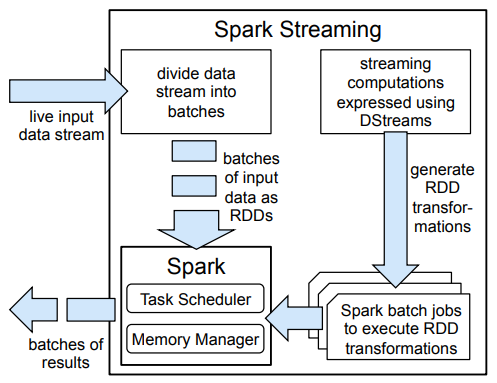
\includegraphics[width=\linewidth]{sparkstreaming}
        \caption{High-level overview of the Spark Streaming system\cite{Zaharia:2013:DSF:2517349.2522737}.}
        \label{fig:sparkstreaming}
\end{figure}
\section{Experiment}
Considered in many fault-tolerant models the data stored in HDFS are necessary to be replicated, and inspired by the Byzantine fault-tolerant mechanism, like how researchers chose \textit{f} and benchmarked performance using GridMix, we modified the replication factor in the official Hadoop MapReduce program from 2 to 3. To benchmark the system performance under different replication factors, we deployed the TestDFSIO benchmark\cite{testdfsio} to automatically create many files with the same size, then input these files to the system and evaluated three performance measurements of both read and write operations: duration, throughput, and average IO rate, as shown in table \ref{tab:title}. In figure \ref{fig:hadoop} we can see those three measurements printed on the terminal after job execution finished.
\begin{table}[ht]
\centering
\caption{Conditions and measurements in our experiment.}
\resizebox{\linewidth}{!}{
\begin{tabular}{ |c|c|c|c| } 
\hline
conditions &\multicolumn{3}{c|}{measurements}\\
\hline
individual file size & duration & throughput & average  IO  rate \\ 
\hline
split number& duration & throughput & average  IO  rate \\ 
\hline
\end{tabular}
}
 \label{tab:title} 
 \end{table}
\subsection*{Environment Setup}
In our experiment, we kept other system parameters unchanged and only modified the DFS configuration file which controlled the replica number in MapReduce job execution.\par

All codes were written in Java and all the tasks were evenly allocated and executed on 10 desktops (1 NameNode, 7 DataNodes) running Linux operating systems with 32GiB System memory and Intel(R) Xeon(R) CPU E5-2650 v2 @ 2.60 processors. The HDFS platform had already been installed on these machines.

\subsection*{Experiment Design}
All programs took the same input files in TXT format, the application main functionality was inherited from the classical WordCount example: first map tasks read sentences line by line and then an object called \textit{StringTokenizers} split them into separate word (symbols and punctuation were omitted), finally, the reduce tasks counted words frequency and stored to values.
\section{Data Collection}
TestDFSIO is a test available in Hadoop distribution for the IO throughput of the cluster. It provides 1:1 mapping from files to map tasks. It is easy to use, command \textit{-write} creates sample input files, \textit{-read} reads them, and \textit{-clean} deletes the test outputs that stored in HDFS. The log results are stored in the local file directory specified by command \textit{-resFile}.\par

The performance of a framework was assessed by the task processing duration and IO rates. A model was considered more efficient and with better performance if it spent less processing time or had higher throughput\&average IO rates.
\section{Data Analysis}

For the same amount of data (30GB), in one group, we increased single file size from 1GB to 3GB while keeping the number of 10 files unchanged and thus obtained \ref{fig:ds0}. In the other group, we increased the number of input splits from 10 to 30 while keeping each file the same size (1GB).
\begin{figure}[htp]
    \centering
        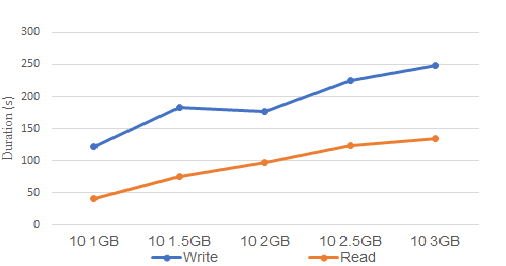
\includegraphics[width=\linewidth]{ds0}
        \caption{Duration when increase individual file size.}
        \label{fig:ds0}
\end{figure}
\begin{figure}[htp]
    \centering
        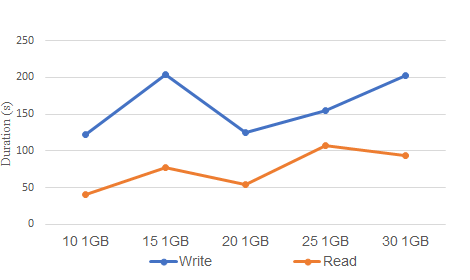
\includegraphics[width=\linewidth]{dn0}
        \caption{Duration when increase split number.}
        \label{fig:dn0}
\end{figure}

When the system replication factor was 2, as shown in figure \ref{fig:ds0} and \ref{fig:dn0}, processing duration is tested by changing either the input file split size or number. In figure \ref{fig:ds0}, though experiences a little fluctuation during the experiment period, the overall duration trend is near-linear proportional to input split size. The differences between these two figures are obvious. First, in both cases the duration of the write operation is about two times that value of the read operation, indicating write is more time consuming than read. Second, for the same amount of data, splitting them into more files slightly reduces the total time spent on operations (the value difference is about 50 seconds and the line slopes in figure \ref{fig:dn0} are smaller than that in figure \ref{fig:ds0}, which means the lines are more "flat").
\begin{figure}[htp]
    \centering
        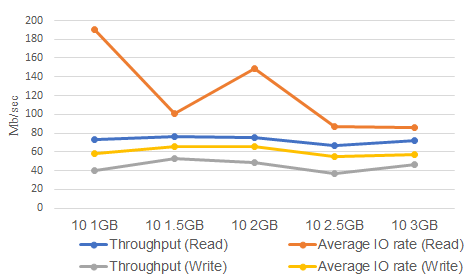
\includegraphics[width=\linewidth]{ts0}
        \caption{Throughput and average IO rates when increase individual file size.}
        \label{fig:ts0}
\end{figure}
\begin{figure}[htp]
    \centering
        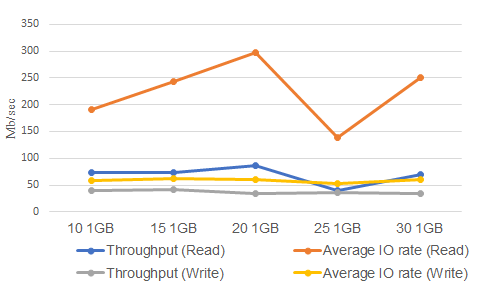
\includegraphics[width=\linewidth]{tn0}
        \caption{Throughput and average IO rates when increase split number.}
        \label{fig:tn0}
\end{figure}

Then we tested the throughput and average IO rate also by applying those two input split changes. As indicated by figure \ref{fig:ts0} and \ref{fig:tn0}, the read operations process more data per unit time than write, and for both figures, the lines represent the average IO rate of read operation fluctuate most, which means this measurement is less stable and more likely to be influenced by input changes, while other values remain relatively stable during the process (but still, every second read processes more data than write). Overall, it is hard to tell which method is better in this case because the differences between the two figures are not obvious.
\begin{figure}[htp]
    \centering
        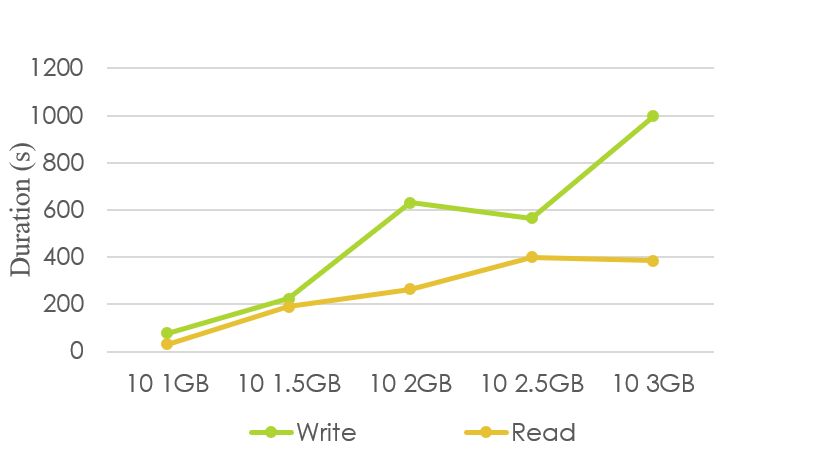
\includegraphics[width=\linewidth]{ds}
        \caption{Duration when increase individual file size.}
        \label{fig:ds}
\end{figure}
\begin{figure}[htp]
    \centering
        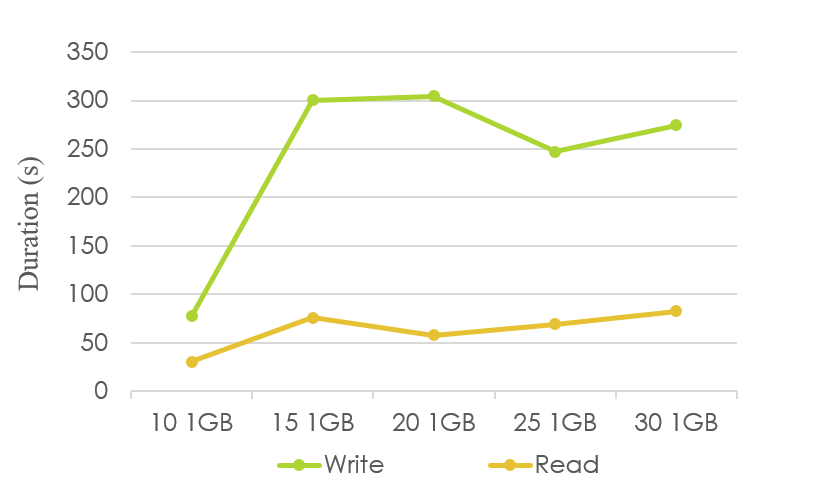
\includegraphics[width=\linewidth]{dn}
        \caption{Duration when increase split number.}
        \label{fig:dn}
\end{figure}

Figures \ref{fig:ds} and \ref{fig:dn} show the performance when replication factor is set to 3, in figure \ref{fig:ds} the duration linearly proportional to the input split size, in fact, if we compare \ref{fig:ds} and \ref{fig:dn} with figures \ref{fig:ds0} and \ref{fig:dn0}, the tendency of duration changes are very similar. However, this time the system with a larger input split size spent approximately 3-6 times the seconds of the system which had an increased split number. Hence this way of input split is not suggested in this model.
\begin{figure}[htp]
    \centering
        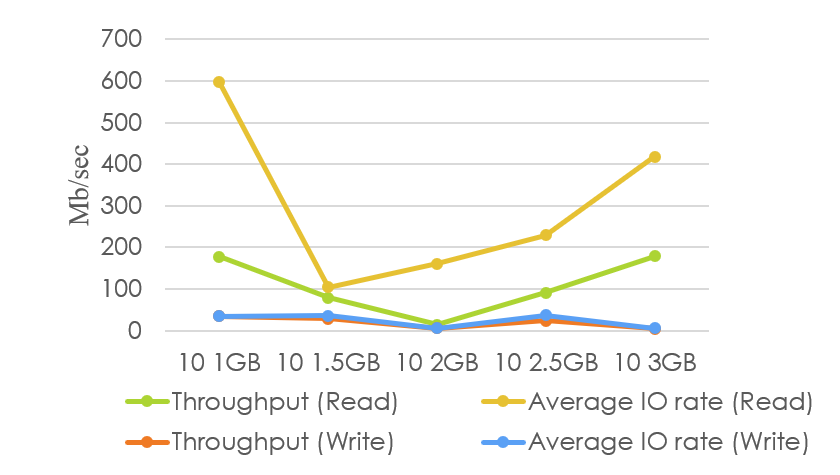
\includegraphics[width=\linewidth]{ts}
        \caption{Throughput and average IO rates when increase individual file size.}
        \label{fig:ts}
\end{figure}
\begin{figure}[htp]
    \centering
        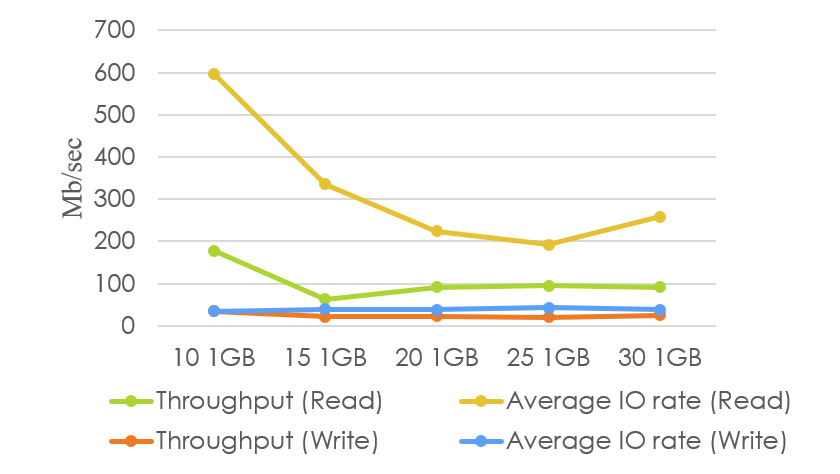
\includegraphics[width=\linewidth]{tn}
        \caption{Throughput and average IO rates when increase split number.}
        \label{fig:tn}
\end{figure}

For the last two figures \ref{fig:ts} and \ref{fig:tn}, the average IO rate of read both decrease first and followed by an increment, this measurement is still the most unstable one. Moreover, compared to the case when the replication factor equals 2, the number of bytes read in every second become 3-5 times of the previous condition, this may happen because when we increase the number of replicas, the system process more files in unit time. 
\section{Discussion}
\subsection*{Reflection}
\subsection*{Future Work}
Future work will be finding out how many replicas should we configure. Because if this value is too small, then once the Namenode fails, the whole system will break and all the data are highly risky of being lost, on the other hand, if this value is set to be too big, those intermediate replications will take a lot of memory space and make it harder to manage and transmit data over the cluster, the less processing time benefit of DFS will also be negatively impacted by more replicas. Thus maintaining a fault-tolerance and performance balance need to be considered when designing new models. 
\subsection*{Conclusion}
In this paper, we first provided an overview of current fault-tolerant mechanisms in Hadoop and Spark, then introduced the fault-tolerant models modified based on the original Hadoop MapReduce framework. Previous works had shown the importance of having multiple duplications as backups in case of defects occurred at low-level nodes. We benchmarked the system performance on three measurements and compared between systems with the replication factor set to 2 and 3 respectively. We also analyzed two methods of splitting input files in order to achieve more efficient read/write executions. Results showed that while the duration time was prolonged when we had more replicas and larger individual file size, the system performance was not heavily impacted by different numbers of replicas or the way data was fed into tasks.\par

Overall, we verified that having more data replicas is a good method to improve system reliability while maintaining the performance on write and read. 
%%%%%%%%%%%%%%%%%%%%%%%%%%%%%%%%%%%%%%%%%%%%%%%%%%%%%%%%%%%%%%%%%%%%%%%%%%%%%%%%
\bibliographystyle{acm}
\bibliography{sample}




\end{document}
